\documentclass{article}
\usepackage[utf8]{inputenc}
\usepackage{hyperref}
\title{keccak preimage}
\usepackage{graphicx}
\usepackage{tikz}
\usepackage{tikz,graphicx}
\usepackage[absolute,overlay]{textpos} 
\usetikzlibrary{decorations.pathmorphing,matrix,decorations.pathreplacing,arrows,decorations.markings}
\usetikzlibrary{fit,calc,shapes,arrows,positioning,shadings,backgrounds,patterns,tikzmark,matrix,spy}
\usetikzlibrary{decorations.markings}

\usepackage[T1]{fontenc}
\begin{document}

\maketitle

\section{Introduction}

The observations based on the following paper : \textbf{Linear Structures: Applications to Cryptanalysis of Round-Reduced Keccak}.

\subsection{2R Keccak-512}

See Fig. 8, for each guess :
we set 
\[
    A[0, 1] = A[0, 0] \oplus \alpha_{0}
\]
\[
    A[2, 1] = A[2, 0] \oplus \alpha_{2}
\]
with $\alpha_0$ and $\alpha_2$ as random constants

Since $A[0,0]$ and $A[2,0]$ have 128 bits. So we have a complexity gain over bruteforce of $2^{128}$. Hence the time complexity $= 2^{512 - 128} = 2^{384}$.

Input degree of freedom : 
\begin{enumerate}
    \item 64 bits from $A[0, 0]$ , 64 bits from $A[2,0]$.
    \item (320 -1) bits from white lanes
    \item 128 bits from $\alpha_0, \alpha_2$
\end{enumerate}

This sums upto 575 bits larger than required 512 bits.

\subsection{2R Keccak-384}

\begin{enumerate}
    \item Attack similar to Keccak-512
    \item Can obtain a linear structure of 256 bits variables from 
    \[
        (A[0, 0], A[0, 1], A[2, 0], A[2, 1])
    \]
    
    \item with : $A[0, 2] = A[0, 0] \oplus A[0, 1] \oplus \alpha_0$
    \item and $A[2, 2] = A[2, 0] \oplus A[2, 1] \oplus \alpha_2$
    \item Hence a linear system of 256-bit equations
    \item Msg satisfying padding rule, need a solution with the last bit of A[2,2] being 1
    \item Time Complexity of Attack $ = 2^{384 - 256 + 1} = 2^{129}$
\end{enumerate}

\textbf{Note :} In the following document WM refers to Willi Meier

\section{Suggestion by WM}

\subsection{Mail : 5 Feb}

Mail contents are : 
\begin{quote}
    I mainly refer to : https://eprint.iacr.org/2016/878
    
    We try to loosen restrictions imposed by linear structures to increase freedom degrees.
    
    An example is 2-round Keccak-384. I refer to Fig. 9. In addition to the colored 6 lanes that are variable, we also keep lanes 3,0 and 3,1 variable, still so that sum of columns is kept constant. Then $\chi$ produces one quadratic lane. We substitute quadratic monomials by 64 linear variables.
    
    We can invert the first row of image (green), and we require that the map to the 6-th green lane is linear (i.e. quadratic part happens to vanish). The probability for this event is about $.75^{64} = 2^{27}$

    Then we have $ 4*64 + 64 + 64 = 384$ variables and the same number of conditions. Solving this linear system has about 1 solution, that we may check by substituting it into 2-round Keccak. Genuine number of freedom degrees is 320, and artficial ones 384. It is likely to find a correct solution in $2^{64} * 2^{27}= 2^{91}$ trials. This case was found in discussion with Meicheng Liu and Jian Guo.
    I believe that something similar (or better) will work for 2-round Keccak-512. In addition to substitution of a quadratic lane by linear variables, we know that variables in same column are linearly related. This means that in quadratic lanes after $\chi$, some linear factors  are essentially "the same".

    The probability of a1*a2 =a1*a3 is 0.75 for any values a1, a2, a3. We substitute monomials of the form a1*a2  and a1*a3 by the same linear variable to get more linear equations that will hold true with reasonable probability. We introduce artificial linear variables economically, so that we don't have more linear variables (genuine and artificial ones) than equations.Details need to be checked.
    
    Wonder whether this could also help, e.g., in 3-round Keccak-256 in \url{https://tosc.iacr.org/index.php/ToSC/article/view/802}.
    
    An issue is how far these observations extend to improve 3 round preimages of Keccak-384 and Keccak-512, as described in Sect. 6.3.
    
    As complexities of known preimages of 4-round Keccak-512 are still close to $2^{512}$, there is some slight hope that we might reach 4 rounds for this case.
    
    Do you have any comments on this?
    \end{quote}
    
    \begin{enumerate}
        \item Here in addition to Keccak-384 setting for 2 Round attack.
        \item In Fig. 9 we keep lanes (3, 0) and (3, 1) also as variables
        \item $A[3, 1] = A[3, 0] \oplus \alpha_3$ (so that sum of columns remains constant)
        \item Linear structure of 320-bit :
        \item $( A[0, 0], A[0, 1], A[2, 0], A[2, 1], A[3, 0] )$
        \item A quadratic term is introduced after 1st $\chi$ by product of $(2, 0), (3, 1)$ as both are variables.
        \item For this we substitute quadratic monomials by 64 linear variables.
        \item Now next problem was for last round : $(\chi o \iota)^{-1}$
        \item For the green lane of second row, this happens to be linear with probability $= 0.75$
        \item For 64 slices, this $= 0.75^{64}$, which adds $2^{27}$ trials
        \item Complexity comes out to be $ = 2^{64} * 2^{27} = 2^{91}$ trials.
        \item \textbf{ Comments : }
        \begin{enumerate}
            \item Any issue of Linear independent variable for solution of equations?
            \item Otherwise the analysis is fine here.
        \end{enumerate}
    \end{enumerate}
    \subsection{Suggestion for Keccak-384, 2R}
\begin{enumerate}
    \item \textbf{Note :} After verification this comes out to be incorrect
    \item Same as the setting introduced by WM for 2R Keccak-384 where we keep (3,0) and (3,1) also as variables
    \item Here we introduced a new variable for each quadratic term
    \item The suggestion here is for reducing the trials due to the last round linear $\chi$ inversion.
    \item Instead of inverting $\chi$ for 6th green lane as suggested by WM we can do something like this :
    \item \label{ob2}\textbf{Observation :} When only one output bit is known after $\chi$ step, then the corresponding input bits have $2^4$ possibilities. A way to fix the first output bit to be the same as input bit and the second bit as $1$. It is shown in the Figure~\ref{chi_inv2}.
\begin{figure}[ht]
\begin{center}
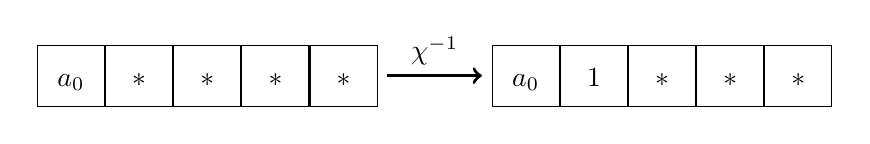
\begin{tikzpicture}[ampersand replacement=\&]
\matrix (m1) [matrix of nodes,
nodes={inner sep=5pt,text width=0.5cm,align=center,minimum height=.5cm, draw,text height=1em,text depth=.2em}
]{
	$a_0$ \& $*$ \& $*$ \& $*$ \& $*$\\
};

\matrix (m2) [right = 1.2cm of m1, matrix of nodes,
nodes={inner sep=5pt,text width=0.5cm,align=center,minimum height=.5cm, draw,text height=1em,text depth=.2em}
]{
	$a_0$ \& $1$ \& $*$ \& $*$ \& $*$\\
};
\draw[->, very thick] (m1)-- node[above, pos=0.5] {$\chi^{-1}$} (m2);
\end{tikzpicture}
\end{center}
\caption{Computation of $\chi^{-1}$\label{chi_inv2}}
\end{figure}
    \item Here in Fig. ~\ref{chi_inv2}, we fix the lane adjacent to 6th green lane as $1$ before $\chi$ operation. If this is assumed then the 6th lane is inverted as it is and seems like a constant.
    \item No. of variables : 5 lane variables + 1(substitute for quadratic terms) and 6 linear conditions. So we Linear structure : $(A[0,0], A[0,1], A[2, 0], A[2,1], A[3,0])$
    \item White lane (constants) : 5 lanes and $64*3$ bits from $\alpha_0, \alpha_2, \alpha_3$
    \item So the degree of freedom is much larger than required 384 bits.
    \item We just want a solution with last bit of $A[2,2]$ being 1.
    \item Time complexity = $2^{384 - (64*5) + 1} = 2^{65}$
    \item If this turns out to be correct then we have a much better attack than proposed by us in our indocrypt-2018 paper with complexity of $2^{88}$
    \item Please verify/correct this. If this is correct then something similar can also be applied to Keccak-512.
\end{enumerate}

\subsection{WM mail : 08/02/19}
For 2R Keccak-512 : 
\begin{enumerate}
    \item 1st row of hashes can be inverted
    \item For 2nd row, we know 3 consecutive outputs. So as in paper (Linear Structures: Applications to Cryptanalysis of Round-Reduced Keccak)
    \item Using table 4, we know that for 3 consecutive output bits in a row known we get 2 linear equations.
    \item For 64 lane size, we get $ 2*64 = 128 $ equations.
    \item For the Message : we keep columns 0, 1, 2 and 3 as variables
    \item \[ A[0, 1] = A[0, 0] \oplus \alpha_0 \]
        \[ A[1, 1] = A[1, 0] \oplus \alpha_1 \]
         \[ A[2, 1] = A[2, 0] \oplus \alpha_2 \]
         \[ A[3, 1] = A[3, 0] \oplus \alpha_3 \]
    \item This state produces quadratic variables after $\pi \circ \rho \circ \theta$.
    \item  This creates 3 quadratic lanes after $\chi$ of 1st round, caused by product of [0,0] with [1,1], and [1,0] with [2,1], and [2,0] with [3,1].
    \item Substitute each of the above quadratic variable by a new linear variable.
    \item So we need $3*64$ new linear variables
    \item Degree of freedom : 
    \begin{enumerate}
        \item Linear structure : $( A[0,0], A[1,0], A[2,0], A[3,0] )$ i.e. $4*64$ variables
        \item Artificial : $3*64$ linear variables
        \item Adds upto overall : $7*64$
    \end{enumerate}
    \item No. of linear conditions :
    \begin{enumerate}
        \item 5 from inversion of chi from the first row of hashes
        \item 2 from inversion of chi from 3 consecutive output bits of hash
        \item Hence, overall 7 equations
    \end{enumerate}
    \item We have 7 linear variables and 7 equations so we can expect to find a solution.
    \item But Actual degree of freedom : 4 i.e. $( A[0,0], A[1,0], A[2,0], A[3,0] )$ and 8 conditions on the final hash (8 lanes)
    \item So, no. of trials $= 2^{512 - 4*64} = 2^{64*4} = 2^{256}$
\end{enumerate}

\end{document}